\chapter{Vulnerability Analysis}

\section{Overview}

This section describes the \textbf{Vulnerability Analysis} activities performed during the penetration testing process.
\\

Vulnerability Analysis is the process of identifying weaknesses within systems and applications that could potentially be exploited by an attacker. These weaknesses may include a wide range of issues, such as host and service misconfigurations, outdated software components, or insecure application design.

\section{Automatic Analysis}

\subsection{Nessus}

To identify potential vulnerabilities within the target system, the vulnerability scanner \texttt{Nessus} was used.
\\

As a first step, a \textit{Basic Network Scan} was performed. The scan identified only two vulnerabilities: one classified as \textbf{medium risk} and one classified as \textbf{low risk}.

\begin{figure}[H]
    \centering
    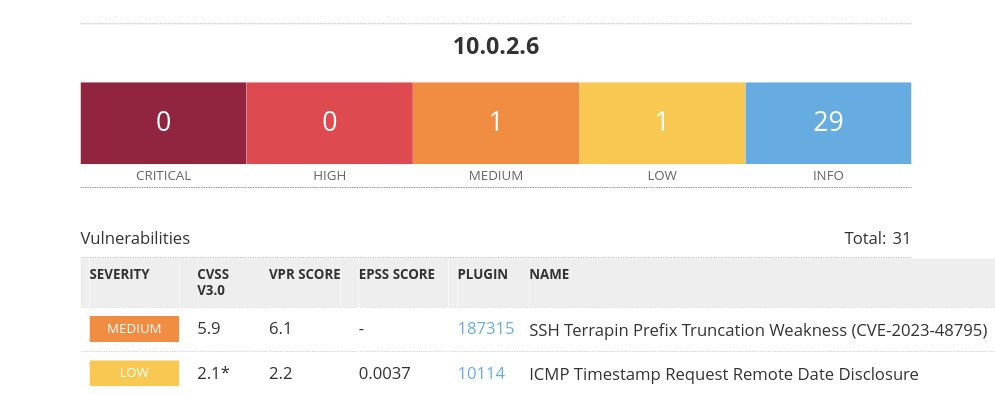
\includegraphics[width=0.75\linewidth]{GlobalAssets/nessus_basic_scan.png}
    \caption{\texttt{Nessus} Basic Network Scan}
    \label{nessusbasic}
\end{figure}


Afterwards, an advanced scan was performed using the following configuration:

\begin{description}
    \item[\textbf{Policy}] Web Application Test;
    \item[\textbf{Port Scan}] All Ports;
    \item[\textbf{Override Normal Accuracy}] Show Potential False Alarms;
    \item[\textbf{Assess Component Install for Potential Vulnerabilities}] Enabled;
    \item[\textbf{Perform Thorough Tests}] Enabled;
    \item[\textbf{Try All HTTP Methods}] Enabled;
    \item[\textbf{Attempt HTTP Parameter Pollution}] Enabled.
\end{description}

The advanced scan identified additional families of vulnerabilities: \textbf{3 critical-risk}, \textbf{11 high-risk}, \textbf{13 medium-risk}, and \textbf{0 low-risk}.
\\

\begin{figure}[H]
    \centering
    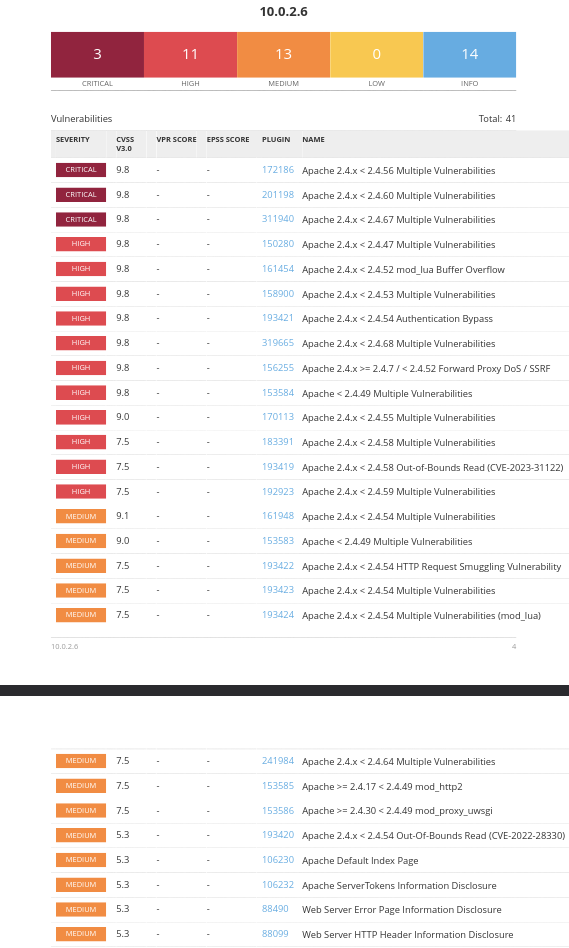
\includegraphics[width=0.75\linewidth]{GlobalAssets/nessus_advanced.png}
    \caption{\texttt{Nessus} Advanced Web Application Test}
    \label{nessusadvanced}
\end{figure}

A complete report generated by \texttt{Nessus} is provided as an attachment; The identified critical vulnerabilities are primarily related to the outdated version of the \texttt{Apache} web server discovered during the previous enumeration phase.
\\

\subsection{Nikto}

A scan on the Web Server was performed with \texttt{Nikto}. The scan confirmed the Nessus findings:

\begin{figure}[H]
    \centering
    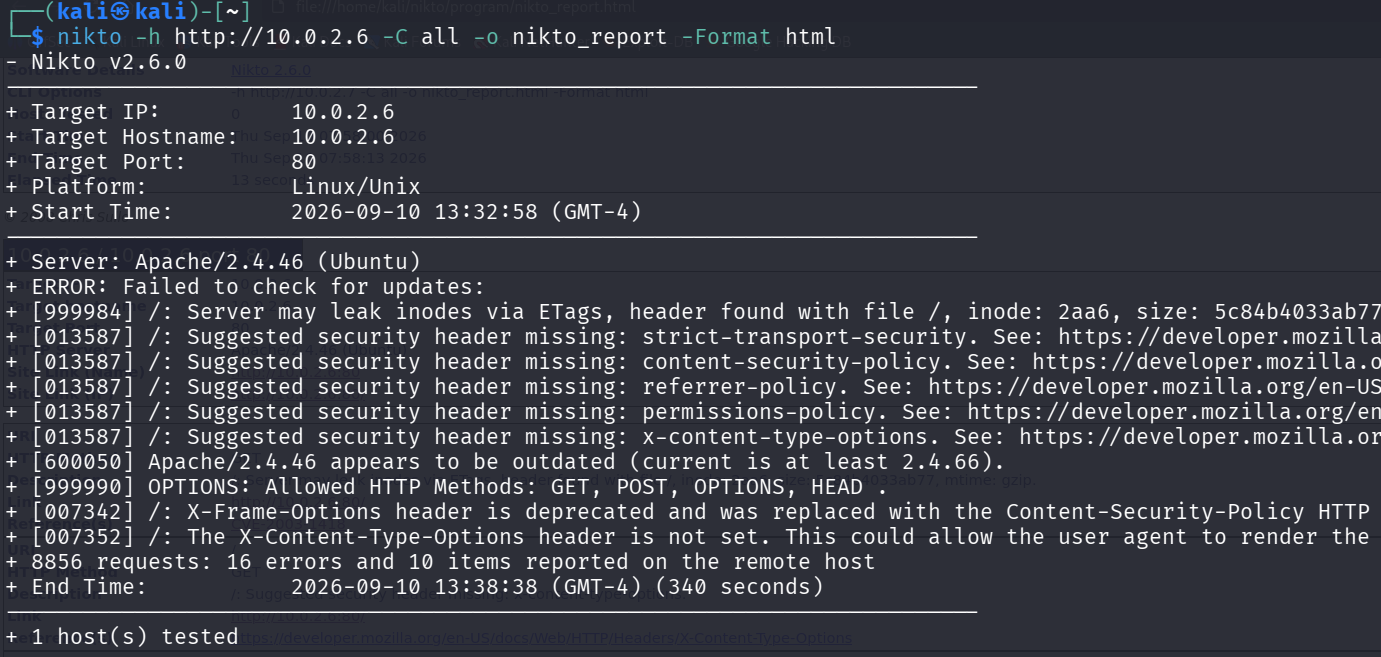
\includegraphics[width=0.75\linewidth]{GlobalAssets/niktoscan.png}
    \caption{Nikto Scan Output}
    \label{niktoscan}
\end{figure}

In addition, \texttt{Nikto} found a new vulnerability identified with \textbf{CVE-2003-1418}. However this vulnerability refers to Apache HTTP Web Server 1.3.22 through 1.3.27, which is an earlier version than the current version running on the target. Therefore the vulnerability is excluded from the final report.
\\

The complete Nikto report is available as an attachment.

\subsection{WafW00f}

To check for the presence of Web Application Firewalls, a scan with WafW00f was executed:

\begin{figure}[H]
    \centering
    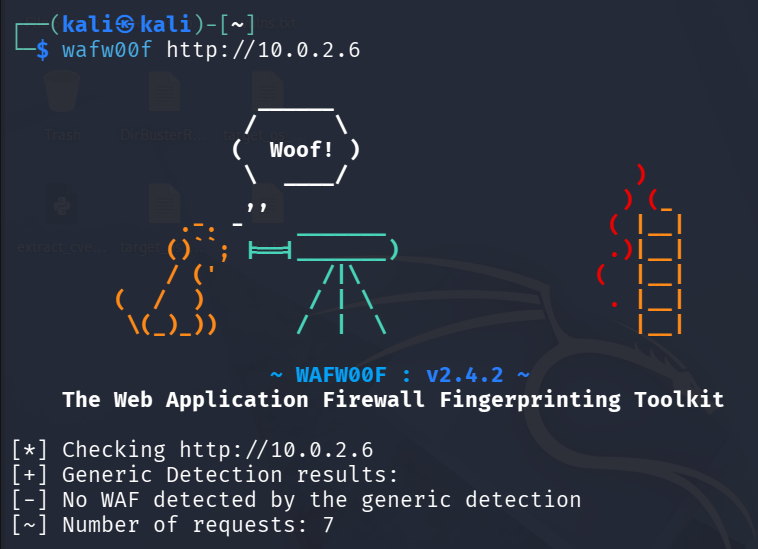
\includegraphics[width=0.50\linewidth]{GlobalAssets/woof.png}
    \caption{WafW00f scan}
    \label{waf}
\end{figure}

However, the target isn't running any Web Application Firewall.

\section{Manual Analysis}

\subsection{Exploit Database Analysis}

To identify additional vulnerabilities that may not have been detected during the automated analysis, the \textit{Exploit Database} was manually consulted. The search was performed using the service and operating system information identified during the \textbf{Intelligence Gathering} phase.
\\

The following information was obtained about the target host:
\begin{itemize}
\item Port \texttt{22} is open and exposes \texttt{OpenSSH 8.4p1};
\item Port \texttt{80} is open and exposes \texttt{Apache HTTP Server 2.4.46};
\item The target system is running a \textit{Linux Ubuntu} operating system with a kernel version between \texttt{4.15} and \texttt{5.19}.
\end{itemize}

The first search was performed using the identified \texttt{OpenSSH 8.4p1} version. No additional vulnerabilities relevant to the target configuration were identified in the \textit{Exploit Database}:
\\

\begin{figure}[H]
\centering
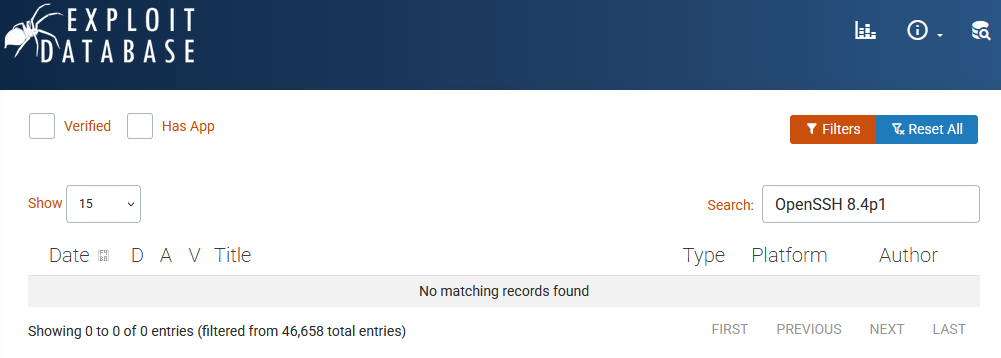
\includegraphics[width=0.75\linewidth]{GlobalAssets/opensshnovuln.png}
\caption{\texttt{OpenSSH 8.4p1} search results in the Exploit Database}
\label{opensshexploitdb}
\end{figure}

A second search was performed for \texttt{Apache HTTP Server 2.4.46}. This search returned an entry associated with \textbf{CVE-2021-44790}. The vulnerability, however, had already been identified by \texttt{Nessus} during the automated vulnerability analysis:
\\

\begin{figure}[H]
\centering
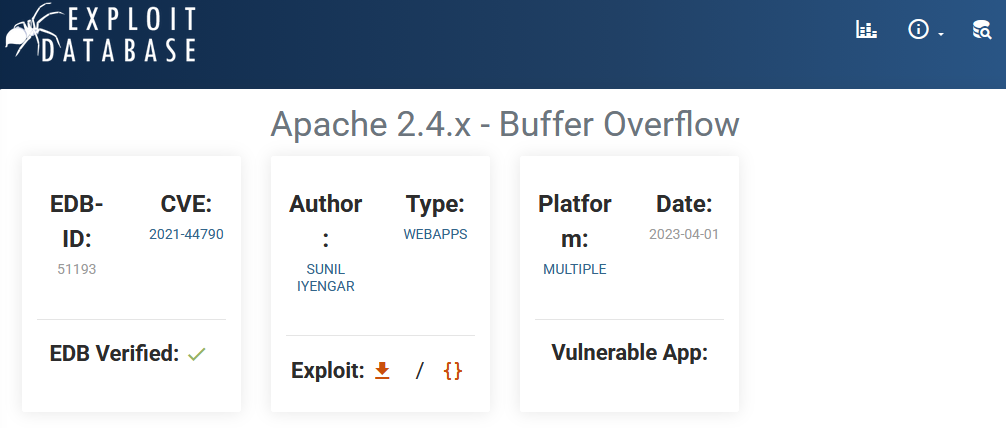
\includegraphics[width=0.75\linewidth]{GlobalAssets/apachemanualscan.png}
\caption{\texttt{Apache HTTP Server 2.4.46} search results in the Exploit Database}
\label{apacheexploitdb}
\end{figure}

Finally, the search was extended to the identified Linux kernel version range. This analysis revealed an additional vulnerability, \textbf{CVE-2018-18955}, which affects Linux kernels within the identified version range. The vulnerability can be exploited by a local, unprivileged user to achieve \textbf{local privilege escalation}:
\\

\begin{figure}[H]
\centering
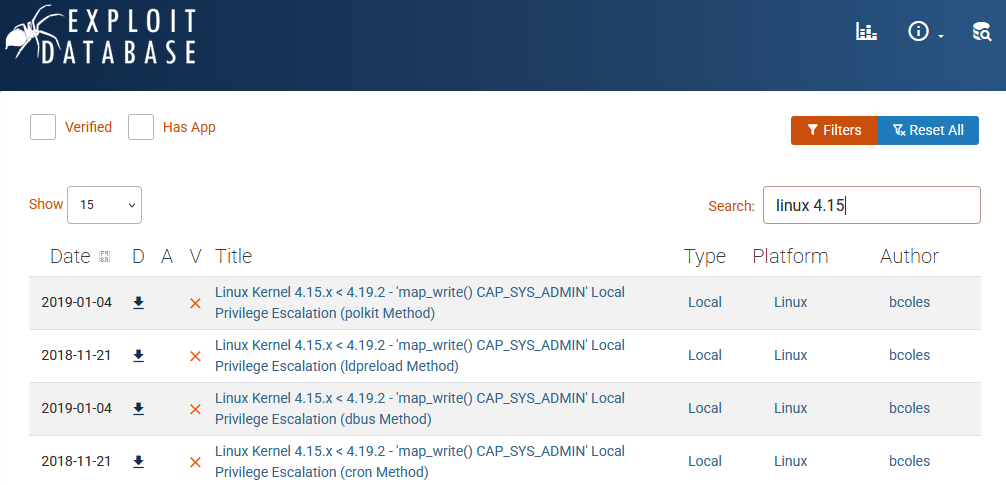
\includegraphics[width=0.75\linewidth]{GlobalAssets/llinuxvulnedb.png}
\caption{Linux kernel search results in the Exploit Database}
\label{linuxexploitdb}
\end{figure}

Unlike the vulnerabilities identified during the automated analysis, \textbf{CVE-2018-18955} was not detected by \texttt{Nessus} and was therefore added as a finding resulting from the manual analysis.

\subsection{Web App Manual Analysis}

As reported in the \textbf{Intelligence Gathering} phase, the following directories and files were identified within the Web App:

\begin{itemize}
\item Directory \texttt{/} --- response code \texttt{200};
\item Directory \texttt{/blog-post/} --- response code \texttt{200};
\item Directory \texttt{/blog-post/archives/} --- response code \texttt{200};
\item Directory \texttt{/blog-post/uploads/} --- response code \texttt{200};
\item Directory \texttt{/tasks/} --- response code \texttt{200};
\item Directory \texttt{/icons/} --- response code \texttt{403};
\item Directory \texttt{/icons/small/} --- response code \texttt{403};
\item Directory \texttt{/server-status/} --- response code \texttt{403};
\item File \texttt{randylogs.php} --- located in \texttt{/blog-post/archives/} with response code \texttt{200};
\item File \texttt{tasks\_todo.txt} --- located in \texttt{/tasks/} with response code \texttt{200}.
\end{itemize}

Some of the discovered files may contain \textbf{sensitive information} that could be useful during the assessment.
\\

By accessing the file \texttt{tasks\_todo.txt}, additional information was disclosed:

\begin{figure}[H]
\centering
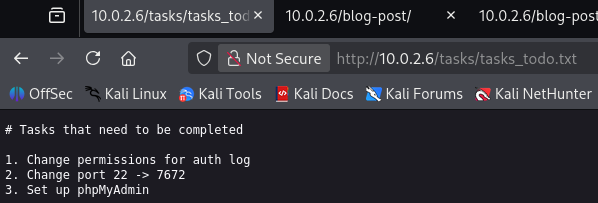
\includegraphics[width=0.75\linewidth]{GlobalAssets/taskstodo.png}
\caption{\texttt{tasks\_todo.txt} content}
\label{taskstodo}
\end{figure}

The content of \texttt{tasks\_todo.txt} suggests the presence of a \textbf{potential misconfiguration} involving the \texttt{auth.log} file. This file is a Linux system log responsible for recording authentication-related events, including:

\begin{itemize}
\item User login and logout events;
\item SSH access attempts;
\item \texttt{sudo} command usage;
\item Failed authentication attempts;
\item \texttt{PAM} (\textit{Pluggable Authentication Modules}) activity;
\item User account modifications;
\item Authentication errors.
\end{itemize}

Another interesting finding is the \texttt{randylogs.php} file. However, attempting to access it directly did not return any information or visible output.
\\

The lack of a response suggests that the PHP script may require an input parameter before it performs its intended function. This is a reasonable assumption given the filename, which indicates that the script is likely related to log retrieval, and the fact that accessing it without any parameters produced an empty response.
\\

To identify the parameter expected by the application, \texttt{wfuzz} was used to perform parameter fuzzing with the wordlist \texttt{/usr/share/wordlists/dirb/big.txt}. In addition, responses with a length of zero were filtered out using the \texttt{--hl} option.
\\

Finally, \texttt{/var/log/auth.log} was considered a potential file that \texttt{randylogs.php} might be intended to access, both because the name of the PHP script suggests that it performs some actions involving log files and because \texttt{auth.log} was explicitly mentioned in \texttt{tasks\_todo.txt}.
\\

This file path was therefore used to determine whether the application accepted a parameter that could be used to retrieve the log file:

\begin{figure}[H]
\centering
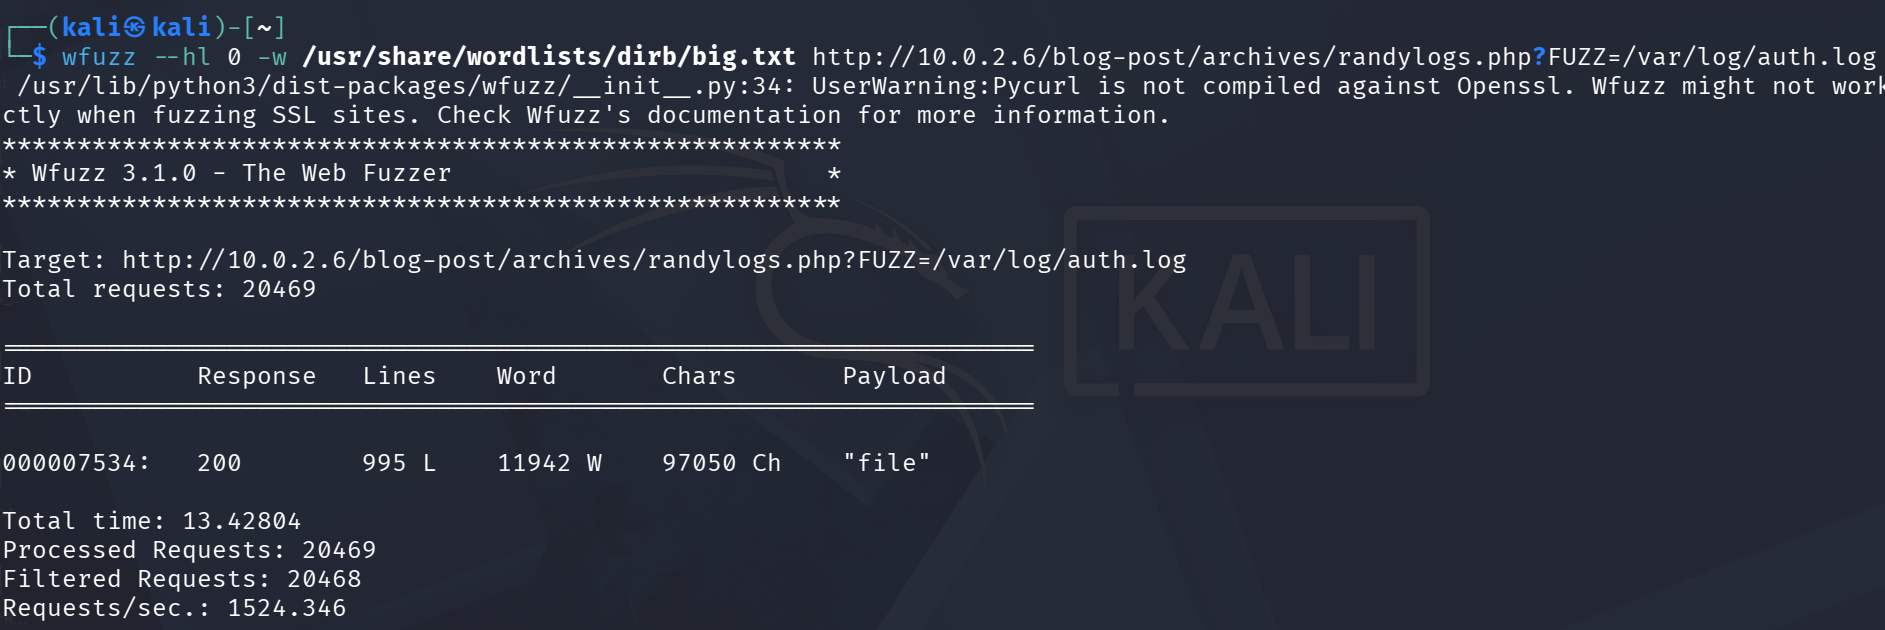
\includegraphics[width=0.75\linewidth]{GlobalAssets/randylogsphpfuzz.png}
\caption{\texttt{randylogs.php} parameter fuzzing}
\label{randylogsfuzzing}
\end{figure}

The output of \texttt{wfuzz} suggests that the parameter \texttt{file} is the one required by the PHP script.
\\

At this point, the observed behavior suggests the presence of a \textbf{potential Local File Inclusion (LFI) vulnerability}. The application appears to accept a user-controlled file path through the \texttt{file} parameter, which may allow the PHP script to access files located on the underlying filesystem. However, the vulnerability can only be confirmed by successfully retrieving a local file through the identified parameter.
\\

Accessing \texttt{http://10.0.2.6/blog-post/archives/randylogs.php?file=/var/log/auth.log} successfully displays the contents of the \texttt{/var/log/auth.log} file, \textbf{confirming the presence of the LFI vulnerability}.

\begin{figure}[H]
\centering
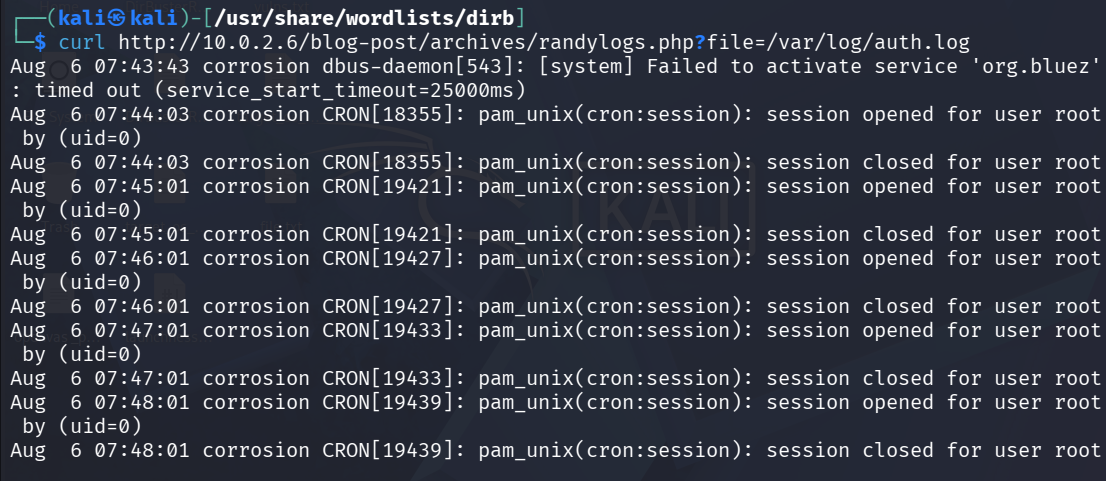
\includegraphics[width=0.75\linewidth]{GlobalAssets/authlogcontent.png}
\caption{\texttt{auth.log} file content}
\label{authlogcontent}
\end{figure}

At this point, it is known that the \texttt{/var/log/auth.log} file contains information about \textbf{SSH authentication attempts}. Since the \texttt{randylogs.php} script can read the contents of \texttt{/var/log/auth.log}, it may be possible to leverage this behavior to achieve \textbf{Remote Code Execution (RCE)} through log poisoning.
\\

In order to test for RCE, an attempt can be made to inject PHP code through the username field during an SSH login. If the supplied input is written to \texttt{/var/log/auth.log} and the resulting log file is subsequently included by \texttt{randylogs.php}, the PHP code may be interpreted by the web server:

\begin{figure}[H]
\centering
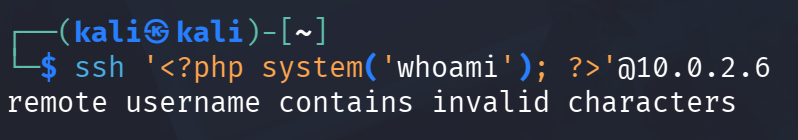
\includegraphics[width=0.75\linewidth]{GlobalAssets/sshinvalidchar.png}
\caption{SSH RCE attempt}
\label{sshrce}
\end{figure}

However, recent SSH implementations do not allow the required characters to be entered through the username field, preventing this particular method of injecting PHP code into the authentication log.
\\

Since the machine allows SSH connections, \textbf{SFTP} (\textit{SSH File Transfer Protocol}) can instead be used as an alternative method to introduce the required input into the target system. The \texttt{curl} utility can be used to interact with the SFTP service and attempt to place the PHP payload in a location that is subsequently processed through the LFI vulnerability:

\begin{figure}[H]
\centering
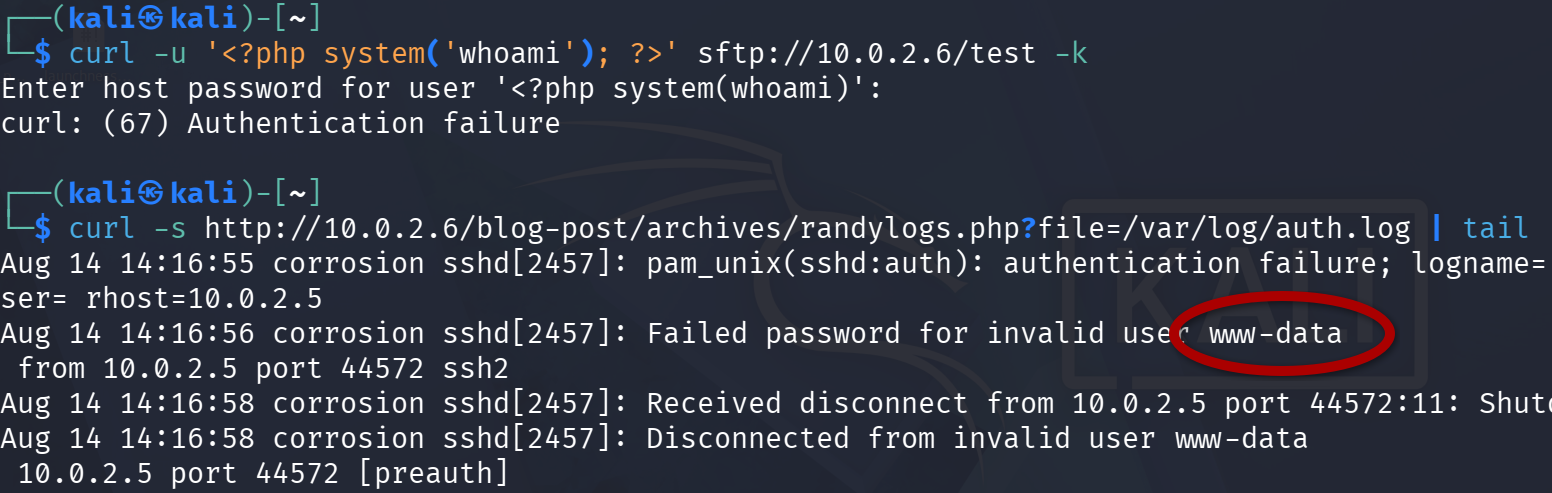
\includegraphics[width=0.75\linewidth]{GlobalAssets/rcesuccess.png}
\caption{SFTP RCE attempt}
\label{sftprce}
\end{figure}

The resulting behavior demonstrates that the LFI vulnerability can be leveraged to achieve \textbf{Remote Code Execution}. The potential impact of achieving \textbf{RCE} will be further investigated during the \textbf{Exploitation phase}.

